\documentclass{standalone}
\usepackage{tikz}
\usepackage{tabularray}
\usepackage{hyperref}
\usepackage{fontawesome7}
\usetikzlibrary{shapes.geometric, arrows}
\tikzstyle{block} = [rectangle, rounded corners,
minimum width=3cm,
minimum height=1cm,
align=center,
draw]

\begin{document}

    \begin{tikzpicture}[scale=1, transform shape, gray]
      \node (energy_out) [block, minimum height = 3cm] at (0,0) {Energy output \\ \footnotesize PVlib};
      \node[anchor= south east, text =blue] at (energy_out.south east) {\footnotesize \href{https://github.com/SjdTl/Magrivoltaics/blob/main/modules/energyOutput.py}{energyOutput.py}};
      \node (energy_used) [block, minimum height = 2cm, anchor=north, yshift=-0.25cm] at (energy_out.south) {Energy usage};
      \node[anchor= south east, text =blue] at (energy_used.south east) {\footnotesize \href{https://github.com/SjdTl/Magrivoltaics/blob/main/modules/energyUsage.py}{energyUsage.py}};
      \node (subtract) [circle, draw, yshift=-0.5cm, xshift=1cm, inner sep = 0pt, minimum size = 0.5cm] at (energy_out.south east) {\Large\textbf{$-$}};
      
      \def\x{7}%
      \path (energy_out.north west)--(energy_out.south west) foreach \j in {1,...,\x} {%
      coordinate [pos=1/(\x + 1)*\j] (y\j)};%
      \foreach \i/\name  in {1/location, 2/azimuth, 3/angle, 4/area, 5/coverage, 6/rated power, 7/efficiency}  %
      \draw[<-] (y\i) -- ++(-2,0) node[anchor=east] (x\i){\name};%
      
      \draw[->] (energy_out.east)  node[anchor=south west] {energy out} -| (subtract.north) node[pos=0.4] {\slash};
      \draw[->] (energy_used.east)  node[anchor=north west] {energy usage} -| (subtract.south) node[pos=0.4] {\slash};
      \draw[->] (subtract.east) -- +(2.25,0) node[midway] {\slash} node[midway, above] {Energy export} node(economic) [block, minimum height=4cm, anchor=west] {Economics};
      \node[anchor= south east, text =blue] at (economic.south east) {\footnotesize \href{https://github.com/SjdTl/Magrivoltaics/blob/main/modules/economics.py}{economics.py}};
        


      \def\x{2}%
      \path (economic.south east)--(economic.south west)
        foreach \j in {1,...,\x} {
          coordinate[pos=1/(\x + 1)*\j] (x\j)
        };
      \foreach \i/\name in {1/subsidy, 2/lifetime} {
        \draw[<-] (x\i) -- ++(0,-1.5) node[anchor=north] (y\i){\rotatebox{90}{\name}};
      }
      \def\x{4}%
      \path (economic.north east)--(economic.south east) foreach \j in {1,...,\x} {%
      coordinate [pos=1/(\x + 1)*\j] (y\j)};%
      \foreach \i/\name/\bus  in {1/LCOE/, 2/ROI/, 3/maintenance/\slash, 4/energy price/\slash}  %
      \draw[->] (y\i) -- ++(2,0) node[anchor=west] (x\i){\name} node[midway] {\bus};%

      \draw (-3,1.75) rectangle (9.5,-5);
      \node[anchor=south west, above right] at (-3,-5) {\Large Interface \faPython};
    \end{tikzpicture}

\end{document}


flow
